\section{Experimental Results}

We compared the performance of our simple linear GP to a variant that replaced the tag-accessed memory with memory indexed with direct arguments (which is more akin to memory access in traditional linear GP~\citep{brameier_linear_2007}).
We evolved programs using the lexicase parent selection algorithm~\cite{helmuth_solving_2015} to solve five problems from Helmuth and Spector's program synthesis benchmark suite~\citep{helmuth_general_2015}: number IO, smallest, median, grade, and for loop index.
For each problem, we added custom instructions to the instruction set that facilitated loading test case inputs into memory and returning program responses. 
We used the same training and testing sets when evaluating programs as Helmuth and Spector in~\citep{helmuth_general_2015}.
We measured performance by counting the number of successful runs (\textit{i.e.}, runs that produced a perfect solution).%, and we tested for statistical significance using Fisher's exact test (with a significance threshold of 0.05).

For each experimental condition, we evolved 50 replicate populations of 500 individuals (for 100 generations for the number IO problem and 500 generations for all other problems), giving each replicate a unique random number seed.
We propagated programs asexually and applied mutations to offspring (single-instruction insertions, deletions, and substitutions at a per-instruction rate of 0.005 each and multi-instruction sequence duplications and deletions at a per-program rate of 0.05). 
The relative success of these two memory-indexing techniques is influenced by how (and at what rate) we mutate instruction arguments.
As such, we mutated tag-based arguments (per-bit) and traditional arguments (per-argument) at the following ten rates: 0.0001, 0.001, 0.0025, 0.005, 0.0075, 0.01, 0.025, 0.05, 0.075, and 0.1. 
See our online supplemental material \citep{tag_accessed_memory_supplement_2019} for source code, details on problem-specific configurations (\textit{e.g.}, program evaluation time, \textit{etc.}), and for our more detailed analyses.

\begin{figure}
  \centering
  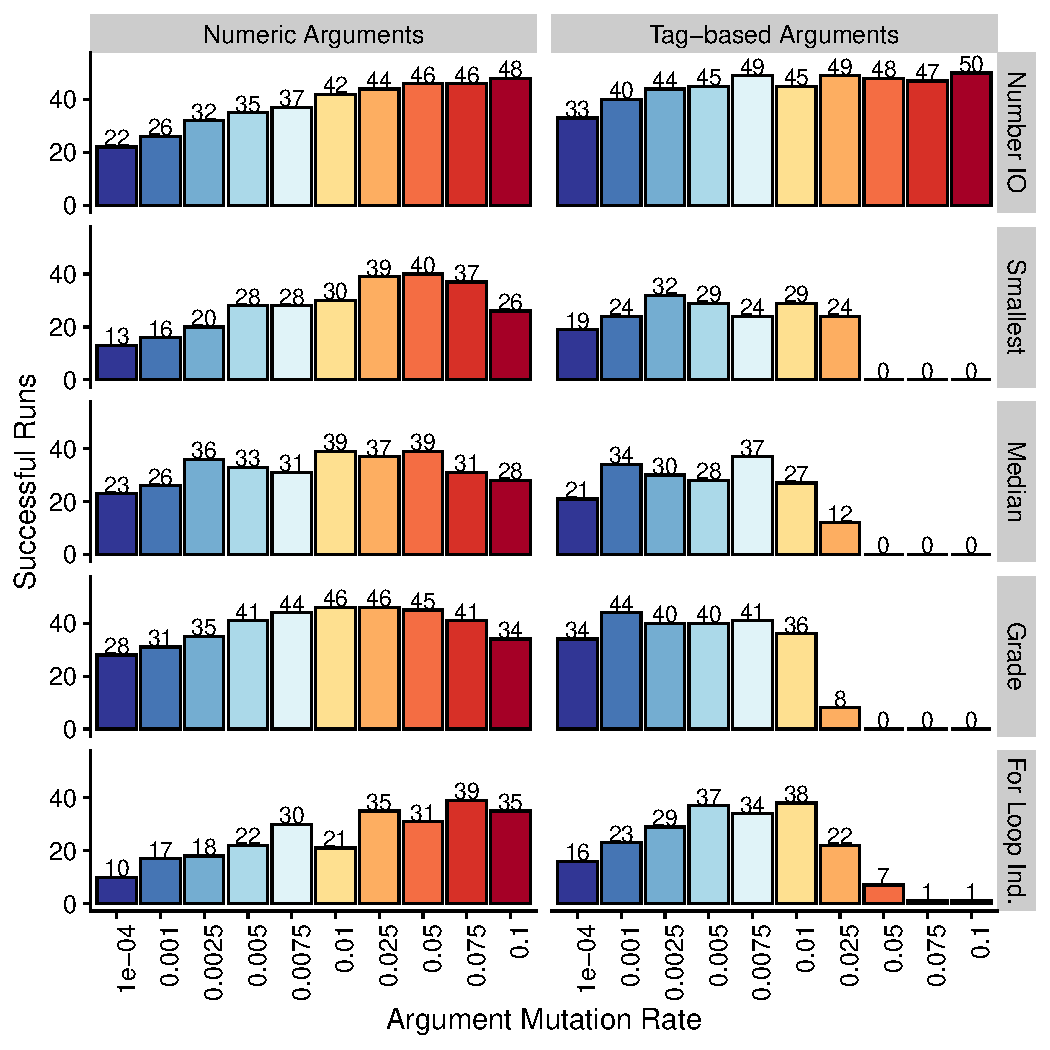
\includegraphics[width=0.75\columnwidth]{chapters/06-tag-access-memory/media/problem-solving-success.pdf}
  \caption{\small 
  \textbf{Number of successful runs} when using our tag-accessed memory (right column) versus using traditional direct-indexed memory (left column) across five problems and ten instruction argument mutation rates (after 100 generations for number IO and 500 generations for all other problems).
  }
  \label{chapter:tag-accessed-memory:fig:successful-runs}
\end{figure}

Figure \ref{chapter:tag-accessed-memory:fig:successful-runs} shows the performance of tag-accessed memory and direct-indexed memory for each problem and mutation rate.
For each problem, we selected the best (most successful) mutation rate for tag-based arguments and the best mutation rate for traditional arguments.
We compared the performance of tag-based arguments and numeric arguments at these ``optimal'' mutation rates, and we tested for we tested for statistical significance using Fisher's exact test (with a significance threshold of 0.05). 
Across all problems, there was no statistically significant difference between tag-based instruction arguments (tag-accessed memory) and numeric instruction arguments (direct-indexed memory).

Figure \ref{chapter:tag-accessed-memory:fig:successful-runs} also seems to indicate that tag-accessed memory is more sensitive to mutation rate than direct-addressed memory. 
Indeed, on the smallest, median, and grade problems, three mutation rates resulted in no solutions in our tag-based argument treatment, whereas all mutation rates in the numeric arguments treatment resulted in at least one solution on all problems.  
This result does not \textit{necessarily} indicate that tag-based arguments are less mutationally robust than numeric arguments.
We mutated numeric arguments at a per-argument rate, and as such, a mutation rate of 0.1 is an expected one mutation for every ten arguments mutated. 
We mutated tag-based arguments at a \textit{per-bit} rate, and as such, a mutation rate of 0.1 is an expected one to two bit flips per mutated tag. 
That is, in practice, the 0.1 per-bit mutation rate for tags is substantially higher than the 0.1 per-argument mutation rate for numeric arguments.
More experiments are needed to quantify tag-based argument and numeric argument sensitivity to mutation.  
% @AML: One more sentence about problem solving success?